%!TEX root = ../research_overview.tex

\section{Energy Efficiency}

\subsection{Link Budget}

\begin{frame}{Link Budget Analysis}

    \only<2-2>{\centering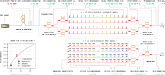
\includegraphics[width=0.85\textwidth]{fig/budget.pdf}}%
    \note<1-1>[item]{Now, let me have a few words on the energy efficiency of the link.}
    \note<2-2>[item]{And this energy estimation really starts from doing a link budget analysis, where I calculate the minimum power required from the comb laser to achieve a target bit error rate, which is 10 to the minus 12. This optical power from the comb will need to traverse a series of optical losses and eventually satisfy the receiver sensitivity.}
    \note<2-2>[item]{And I'd point out that all the optical losses listed here are characterized from measurement data.}

\end{frame}

\subsection{Breakdown}

\begin{frame}{Energy Breakdown}

    \only<1-1>{\centering\includegraphics[width=\textwidth]{fig/energy_compressed.pdf}}%
    \note<1-1>[item]{And then, the laser power consumption is calculated assuming a 15\% wall-plug efficiency, and the total energy consumption here includes not only the laser, but also the driver, receiver, and the thermal control. And it takes about 300 fJ/b with thermal undercut, which is foundry process that selectively removes part of the substrate around and below a device to improve the thermal tuning efficiency. And I'd like to emphasize that this 300 fJ/b is able to carry that data to almost any distance in the system.}

\end{frame}

\subsection{Further Improvement}
\begin{frame}{Return to Metrics}

    \only<1-1|handout:0>{\centering\includegraphics[width=0.8\textwidth]{fig/fom-5_compressed.pdf}}%
    \only<2-2>{\centering\includegraphics[width=0.8\textwidth]{fig/fom-future_compressed.pdf}}%
    \note<1-1>[item]{Now, let me return to this link metric and look at what we have achieved so far, and ask if we can further improve the bandwidth density and energy efficiency.}
    \note<2-2>[item]{And I'd say yes, at least another magnitude, and this is just the beginning, because we have lots of room to improve at both device and integration levels, like for example,}

\end{frame}

\begin{frame}{Paths to Improvement}

    \only<1-1|handout:0>{\centering\includegraphics[width=0.8\textwidth]{fig/path-improve-1_compressed.pdf}}%
    \only<2-2|handout:0>{\centering\includegraphics[width=0.8\textwidth]{fig/path-improve-2_compressed.pdf}}%
    \only<3-3>{\centering\includegraphics[width=0.8\textwidth]{fig/path-improve-3_compressed.pdf}}%
    \note<1-1>[item]{we have disk designs that can be driven faster at an even lower Vpp.}
    \note<2-2>[item]{Our link architecture is very scalable, and I'm working on characterizing this 4 by 32 transmitter array which has this disk design. So that'll be 128 channels at 32 Gb/s, or 4 Tb/s per fiber.}
    \note<3-3>[item]{And also with foundries starting to offer thick silicon nitride layers, we can potentially have an integrated comb source that lowers the optical losses and the energy consumption.}
    \note<3-3>[item]{And this is just the beginning because, as we start to think about a package like this, where it has an integrated comb source, and perhaps the photonics are directly driven by the compute or memory chip, there is a huge space for collaboration, with all the talks about heterogeneous integration and advanced packaging, that in addition to only electronic-photonic integration, how can we make a system with more chiplets integrated on an even larger substrate to further improve the system capabilities.}
    \note<3-3>[item]{With that, I would like to switch gears now and talk about how}

\end{frame}
